\documentclass{article}
\usepackage{amsmath}
\usepackage{graphicx}
\usepackage[a4paper, margin=1in]{geometry}
\usepackage{pgfplots}
\pgfplotsset{compat=1.17}
\usepackage{afterpage}
\usepackage{float}

\title{k-Nearest Neighbors (k-NN) Implementation in Parallel}
\author{Epameinondas Bakoulas and Maria Sotiria Kostomanolaki}
\date{November 2024}

\begin{document}

\maketitle

\begin{abstract}
    This document explains the implementation of the \textbf{k-Nearest Neighbors (kNN)} algorithm in C, both in serial and parallel execution.
    The focus will mainly be on the parallel execution using threads to improve the speed of the execution, assuming that $C=Q$, the
    number of points in the dataset is in the millions and the number of dimensions is in the hundreds.
\end{abstract}

\section{Distance calculation}
In a $d$-dimensional space, the \textbf{Euclidean distance matrix} $D$ between two datasets 
$C$ and $Q$ is calculated as: 
\[
D = \sqrt{C.^2 - 2 C Q^T + (Q.^2)^T}
\]
where $C$ is the \textbf{corpus} dataset with $m$ points and $d$ dimensions, and $Q$ is the \textbf{query} dataset with $n$ points and $d$ dimensions.
$C.^2$ and $Q.^2$ denote element-wise squaring of the matrices and summing along the columns.
The function that implements the above is called \texttt{computeDistances}.

\section{Sequential implementation}
The \texttt{kNNsearch} function finds the k-nearest neighbors for each point in the matrix $Q$.
First, it splits the $Q$ matrix into \emph{blocks} in order to have better control over the memory usage.
Then, it calculates the distances between the points in each \emph{block} and the points in the corpus matrix $C$.
Finally, it finds the k-nearest neighbors for each point in the block.

\section{Parallel implementation}
We will assume $C=Q$ from now on and we will aim to find an \emph{approximate} solution for the k-nearest neighbors problem.

\subsection{Initialization}
We first create a struct called \texttt{Neighbor} that holds an \emph{index} and a \emph{distance}.
The function \texttt{kNN} initializes an $n \times k$ array \texttt{nearestNeighbors} to store the nearest neighbors for each point.
Each element in this array is initialized with a distance of \emph{INFINITY} and an index of $-1$.

\subsection{Splitting data into blocks}
The data points are divided into \emph{blocks} randomly due to memory contsraints. This is achieved using the helper 
function \texttt{shuffleIndices} that takes an array of indices and shuffles them randomly. The first $n / numBlocks$ 
points are assigned to the first block, the next $n / numBlocks$ points to the second block, and so on.

For example, consider the matrix 
\[
C = \begin{bmatrix}
1 & 2 \\
3 & 4 \\
5 & 6 \\
7 & 8 \\
9 & 10 \\
11 & 12 \\
13 & 14 \\
15 & 16
\end{bmatrix}
\]

one possible split into 4 blocks is:
\[
\text{Block 1} = \begin{bmatrix}
1 & 2 \\
11 & 12
\end{bmatrix}, \quad
\text{Block 2} = \begin{bmatrix}
3 & 4 \\
13 & 14
\end{bmatrix}, \quad
\text{Block 3} = \begin{bmatrix}
5 & 6 \\
15 & 16
\end{bmatrix}, \quad
\text{Block 4} = \begin{bmatrix}
7 & 8 \\
9 & 10
\end{bmatrix}
\]


\subsection{Processing blocks}
For each block, we calculate the distances between the points and update the nearest neighbors.
Finding the k-Nearest Neighbors is achieved with the function \texttt{quickSelect}. It takes as input
the neighbors of a point (an array of \texttt{Neighbor}s) and quick selects the distances to find the $k$ nearest neighbors.

The blocks are processed in parallel. Each thread processes a block, until all blocks are processed.

\subsection{Improving the Solution}
The solution is improved by finding distances between points in different blocks using a subset of the points. 
For example, if we combine pairs of blocks by choosing only $50\%$ of the points in random (1 point from each block),
we might get:
\[
\text{Subset from Block 1} = \begin{bmatrix}
1 & 2
\end{bmatrix}, \quad
\text{Subset from Block 2} = \begin{bmatrix}
13 & 14
\end{bmatrix}
\]
The distance matrix can then be used to improve the solutions of both blocks. In the above example, we will find the
distance between the points $[1, 2]$ and $[13, 14]$ and update the nearest neighbors for both points if we end up finding a new
nearest neighbor.

We will repeat this process until all block pairs have been processed. Note that if we process a pair $(i, j)$, we will 
not process the pair $(j, i)$ since the distances are symmetric.

The block pairs are processed in parallel. Each thread processes a block pair, until all block pairs are processed.

\subsection{Analyzing the end results}
The last step is to find the \emph{Recall} and \emph{Queries per second} of the algorithm. Recall is equal to the percentage of the
correct neighbors that we find. It is calculated by comparing the ground truth (exact) solution of the algorithm with the 
approximate solution.
\[
\text{Recall} = \frac{\text{\# correct neighbors}}{\text{total neighbors}}
\]
Queries per second is the number of queries that the algorithm can process in one second. 
\[
\text{Queries per second} = \frac{n}{\text{execution time}}
\]


\section{Benchmarks}
We will display the benchmarks produced from testing the data \emph{sift-128-euclidean}.
It has a total of $n=1,000,000$ points and $d=128$ dimensions, and we find the $k=100$ nearest neighbors.
Tested on a computer with CPU: i5-11400F (6 cores, 12 threads), 16GB RAM, and OS: Linux Mint 22.
The following graph summarizes the benchmarks for different implementations:

\begin{figure}[H]
\centering
\begin{tikzpicture}
    \begin{axis}[
        title={Queries per second vs Recall (4 Threads, sift-128-euclidean)},
        xlabel={Recall (\%)},
        ylabel={Queries per second},
        legend pos=north east,
        ymajorgrids=true,
        grid style=dashed,
        yticklabel style={/pgf/number format/fixed},
        scaled y ticks=false,
        width=0.9\textwidth,
        height=0.3\textheight,
    ]

\addplot[
    color=blue,
    mark=square,
    ]
    coordinates {
    (25.34, 938) (2.22, 11995)
    };
    \addlegendentry{Pthreads}

\addplot[
    color=red,
    mark=triangle,
    ]
    coordinates {
    (26.52, 905) (2.24, 12064)
    };
    \addlegendentry{OpenMP}

\addplot[
    color=green,
    mark=o,
    ]
    coordinates {
    (26.54, 915) (2.24, 11846)
    };
    \addlegendentry{OpenCilk}

\end{axis}
\end{tikzpicture}
\caption{Queries per second vs Recall for different implementations}
\end{figure}

We can see that all 3 implementation produce very similar results.

\end{document}
